% So we make this "beamer" rather than document!

\documentclass[11pt]{beamer}
% For handout add ,handout after 11pt

\usetheme[sectionpage=none,numbering=none]{metropolis}           % Use metropolis theme
	% To do printouts, add ", handout"  after aspectratio.
\usepackage{booktabs}
\usepackage{graphicx}
\usepackage{color}

\title{Unifying Data Science}
\author{\small Nick Eubank}
\date{\vspace*{.3in} \date}


% This is the beginning of a real document!
\begin{document}


\begin{frame}[c]
\maketitle
\end{frame}

\begin{frame}[c]{}
\begin{enumerate}
  \item Provide unified conceptual framework for relating data science tools
  \item Learn causal inference
  \item Get practice developing data science project start-to-finish
\end{enumerate}
\end{frame}

\begin{frame}[c]{How did Data Science become a thing?}

\begin{itemize}
	\pause \item Academic research is organized into silos:
	\pause
	\begin{itemize}
		\item Computer Science
		\item Statistics
		\item Economics
		\item Political science
		\item Engineering
	\end{itemize}
\end{itemize}
\pause $\Rightarrow$ Development of new tools occurred \emph{within} each silo.
\end{frame}


\begin{frame}[c]{Where are we today?}
Very little cross-pollination across silos
\begin{itemize}
	\pause \item Lots of duplication of development.
	\pause \item Every silo has its own vocabulary.
	\pause \item Each silo has focused on the aspects most relevant to their applications. e.g.:
	\begin{itemize}
		\pause \item CS likes to classify things and make predictions, don't care how model works
		\item Social scientists like to make causal statements, don't care about predictive power
	\end{itemize}
\end{itemize}
\end{frame}

\begin{frame}[c]{}
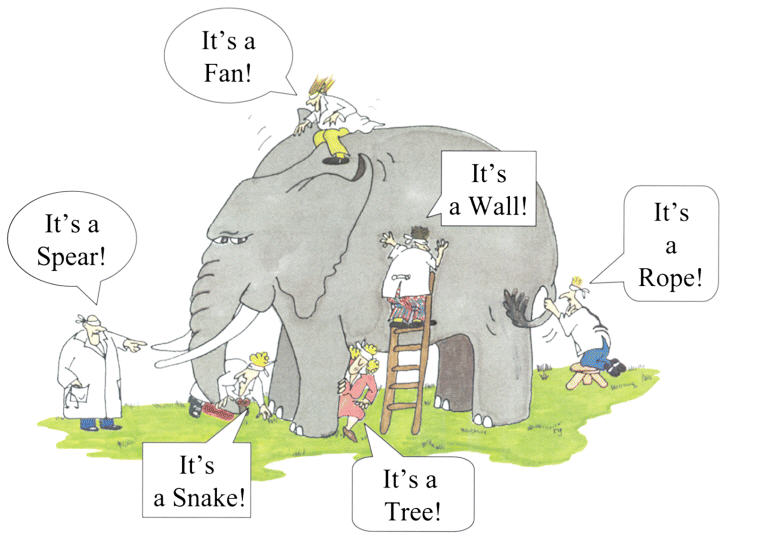
\includegraphics[width=\textwidth]{blindmenelephant.jpg}
$\Rightarrow$ This is where we are \emph{now.}
\end{frame}

\begin{frame}[c]{What is (empirically) Data Science?}
\pause An effort to unify the development of quantitative methods \\
\pause $\rightarrow$ Recognize the elephant
\end{frame}

\begin{frame}[c]{This Class}
Discipline of learning how best to \alert{answer questions} using \alert{quantitative data.}
\end{frame}

\begin{frame}[c]{This Class}
\begin{enumerate}
  \item Introduce a taxonomy of questions \\
  {\color{gray} Descriptive, causal, predictive}
  \pause \item \alert{For each class of questions}, we will discuss the relative strengths and weaknesses of different empirical approaches
  \begin{itemize}
    \pause \item Unsupervised machine learning
    \item Supervised machine learning
    \item Range of causal inference techniques \\
    {\color{gray}e.g. experiments, matching, regression, differences-in-differences}
    \item Other approaches to descriptive analysis
  \end{itemize}
\end{enumerate}
\end{frame}


\begin{frame}[c]{This Class}
The tool you use should be dictated by the question you seek to answer
\end{frame}

\begin{frame}[c]{This Class}
\begin{enumerate}
  \item Provide unified conceptual framework for relating data science tools\\
  \only<2->{\color{gray} Practice generating questions}
  \item Discuss descriptive questions \\
  \only<3->{\color{gray} Relatively brief}
  \item Learn causal inference \\
  {\color{gray} Deep dive -- $\sim$ half the semester}
  \item Discuss prediction \\
  \only<4->{\color{gray} Relative merits of supervised machine learning v. causal methods}
\end{enumerate}
\end{frame}

\begin{frame}[c]{Data Science Project}
Over semester, you will also develop a data science project from start-to-finish
\begin{itemize}
  \item Teams of 2-3, grouped by interest and experience
  \item On topic of your own choosing
\end{itemize}
\pause $\rightarrow$ Nice portfolio piece\\
\pause $\rightarrow$ MIDS first-years: Capstone with training wheels
\end{frame}

\end{document}
